\documentclass[11pt]{article}

% some definitions for the title page
\newcommand{\reporttitle}{Nueral Machine Translation}
\newcommand{\reportdescription}{example}

% load some definitions and default packages
%---------------------------------------------------------------------------
%	PACKAGES AND OTHER DOCUMENT CONFIGURATIONS
%---------------------------------------------------------------------------

\usepackage[twoside]{fancyhdr}
\usepackage{csquotes}

\usepackage[a4paper,hmargin=2.0cm,vmargin=1.0cm,includeheadfoot]{geometry}
% \usepackage{natbib} % for bibliography
\usepackage{biblatex}
\usepackage{tabularx,longtable,multirow,subfigure,caption}%hangcaption
\usepackage{fancyhdr} % page layout
\usepackage{url} % URLs
\usepackage[english]{babel}
\usepackage{graphicx}
\usepackage{rotating}
\usepackage{dsfont}
\usepackage{epstopdf} % automatically replace .eps with .pdf in graphics
% \usepackage{backref} % needed for citations
\usepackage{array}
\usepackage{latexsym}
\usepackage[pdftex,hypertexnames=false,colorlinks]{hyperref} % provide links in pdf (had pagebackref)
\usepackage{booktabs}
\usepackage{wrapfig}
\usepackage{caption}  % Required for \captionof
\usepackage{float} % for H option in figures
\usepackage{amssymb}
\usepackage{amsmath}
\usepackage{amsthm}
\usepackage{mathtools} % for 'dcases*' env.
\usepackage[nottoc]{tocbibind}

%%% Default fonts
\renewcommand*{\rmdefault}{bch}
\renewcommand*{\ttdefault}{cmtt}

%%% Default settings (page layout)
\setlength{\parindent}{0em}  % indentation of paragraph
\setlength{\parskip}{.3em}
\setlength{\itemsep}{0.mm}

\setlength{\headheight}{14.5pt}
\pagestyle{fancy}

\fancyfoot[ER,OL]{\thepage}%Page no. in the left on odd pages and on right on even pages

\fancyfoot[OC,EC]{\sffamily }
\renewcommand{\headrulewidth}{0.1pt}
\renewcommand{\footrulewidth}{0.1pt}
\captionsetup{margin=10pt,font=small,labelfont=bf}

% LISTINGS ammendments
\usepackage{listings}
\usepackage{color}

\definecolor{mygreen}{rgb}{0,0.6,0}
\definecolor{mygray}{rgb}{0.5,0.5,0.5}
\definecolor{mymauve}{rgb}{0.58,0,0.82}

\lstset{ 
  postbreak=\mbox{\textcolor{red}{$\hookrightarrow$}\space},
  backgroundcolor=\color{white},   % choose the background color; you must add \usepackage{color} or \usepackage{xcolor}; should come as last argument
  basicstyle=\footnotesize,        % the size of the fonts that are used for the code
  breakatwhitespace=false,         % sets if automatic breaks should only happen at whitespace
  breaklines=true,                 % sets automatic line breaking
  captionpos=b,                    % sets the caption-position to bottom
  commentstyle=\color{mygreen},    % comment style
%   deletekeywords={...},            % if you want to delete keywords from the given language
%   escapeinside={\%*}{*)},          % if you want to add LaTeX within your code
  extendedchars=true,              % lets you use non-ASCII characters; for 8-bits encodings only, does not work with UTF-8
  firstnumber=1,                % start line enumeration with line 1000
  frame=single,	                   % adds a frame around the code
  keepspaces=true,                 % keeps spaces in text, useful for keeping indentation of code (possibly needs columns=flexible)
  columns=fullflexible,
  keywordstyle=\color{blue},       % keyword style
  language=python,                 % the language of the code
  % morekeywords={*,...},            % if you want to add more keywords to the set
  numbers=left,                    % where to put the line-numbers; possible values are (none, left, right)
  numbersep=5pt,                   % how far the line-numbers are from the code
  numberstyle=\tiny\color{mygray}, % the style that is used for the line-numbers
  rulecolor=\color{black},         % if not set, the frame-color may be changed on line-breaks within not-black text (e.g. comments (green here))
  showspaces=false,                % show spaces everywhere adding particular underscores; it overrides 'showstringspaces'
  showstringspaces=false,          % underline spaces within strings only
  showtabs=false,                  % show tabs within strings adding particular underscores
  stepnumber=1,                    % the step between two line-numbers. If it's 1, each line will be numbered
  stringstyle=\color{mymauve},     % string literal style
  tabsize=2,	                   % sets default tabsize to 2 spaces
  title=\lstname% show the filename of files included with \lstinputlisting; also try caption instead of title
}

% Here, you can define your own macros. Some examples are given below.

\newcommand{\R}[0]{\mathds{R}} % real numbers
\newcommand{\Z}[0]{\mathds{Z}} % integers
\newcommand{\N}[0]{\mathds{N}} % natural numbers
\newcommand{\C}[0]{\mathds{C}} % complex numbers
\renewcommand{\vec}[1]{{\boldsymbol{{#1}}}} % vector
\newcommand{\mat}[1]{{\boldsymbol{{#1}}}} % matrix


\begin{document}

% Include the title page
\begin{titlepage}

    \newcommand{\HRule}{\rule{\linewidth}{0.5mm}} % Defines a new command for the horizontal lines, change thickness here
    
    \center % Center everything on the page
     
    %------------------------------------------------------------------------
    %	HEADING SECTIONS
    %------------------------------------------------------------------------
    
    \textsc{\Large Department of Computing}\\[0.5cm] 
    \textsc{\large Imperial College of Science, Technology and Medicine}\\[0.5cm] 
    
    %------------------------------------------------------------------------
    %	TITLE SECTION
    %------------------------------------------------------------------------
    
    \HRule \\[0.4cm]
    { \huge \bfseries \reporttitle}\\ % Title of your document
    \HRule \\[0.4cm]

    \textit{\reportdescription}
    
    \vspace{2em}

    %------------------------------------------------------------------------
    %	AUTHOR SECTION
    %------------------------------------------------------------------------
    
    \large \emph{Author: Anton Zhitomirskiy}

    \vspace{1em}

    \global\let\newpagegood\newpage
    \global\let\newpage\relax
    
\end{titlepage}

\global\let\newpage\newpagegood

\tableofcontents

\clearpage

\section{Machine Translation}

At the highest level, given a document in source language, produce a translation in a target language.

\subsection{Statistical Machine Translation}

It is a pipeline of the models: Alognment model, Translation model, and Lanugage model.

Uses parallel corpa as its training set. A prallel corpa is that we have aligned sentences: i.e. an english sentence and its corresponding french sentence.

\begin{figure}[H]
    \centering
    \includegraphics*[width=.6\linewidth]{figures/smt-idea.png}
\end{figure}

\begin{itemize}
    \item Parallel dataset - paired sentences between two different languages (we wnat to construct correlations betwene the two sets)
    \item Alignment model - responsible for extracting the phrase pairs    
    \item Translation model - lookup table, what is the porbability of the word `go' appearing in the contex of this target. statistics over large pairs of parallel texts can
    help identify parallel phrases
    \item Corpus of target monolongual corpus - this is used to get n-grams from the data
    \item Language model - contains the probability of target language phrases 
\end{itemize}

\subsubsection{How to perform translations}

\begin{itemize}
    \item The objective is to find $p(t|s)$; given a source sentence, s, we want target sentence, t. Language models can be trained on monolingual data\footnote{todo} that gives us probability of a phrase occurring in that language.
    \item The translation model is the ``objective'' flipped. How likely is the source phrase going to occur given a cnadidate translation t. We will have multiple candidate translations. 
    \item These probabilities/likelihoods are built from statistics of our bilingual parallel corpus.
    \item With this information we can apply Bayes rule to obtain $p(t|s)$.
    \begin{equation*}
        p(t|s) = \frac{p(t)p(s|t)}{p(s)}
    \end{equation*}
    \item p(s) is just a normalising factor. It doesn't contain t so is irrelevant to     obtaining what we're interested in: the actual model
    \item The actual model is the argmaxs. Here - pick the phrase that has the highest
    probability of the product of the 2 terms $p(t)$ (language model) and $p(s|t)$
    (translation model)
\end{itemize}

\subsubsection{Example}

\begin{figure}[H]
    \centering
    \includegraphics*[width=.6\linewidth]{figures/example-translation-1.png}
\end{figure}

The first part is to use the trsnlation model, so given these target phrases which have been built by the alignment model and the probabilities which are in the translation modle, what is the most likely candidate, the most likely translation candidate for this given sole sentence. 

The second part is the lnaguage model itself, which will take each one of these candidates and compute how likley they are to actually appear in target data.

\subsubsection{Downsides}

\begin{itemize}
    \item Sentence Alignment
    
    In parallel corpora single sentences in one language can be translated into
    several sentences in the other and vice versa. Long sentences may be
    broken up, short sentences may be merged. There are even some
    languages that use writing systems without clear indication of a sentence
    end (for example, Thai).

    \item Word Alignment
    
    Is about finding out which words align in a source-target sentence pair

    One of the problems presented is function words that have no clear
    equivalent in the target language. For example, when translating from
    English to German the sentence "John does not live here," the word
    "does" doesn't have a clear alignment in the translated sentence "John
    wohnt hier nicht."

    \item Statistical anomalies
    
    Real-world training sets may override translations of, say, proper nouns.
    An example would be that "I took the train to Berlin" gets mis-translated as
    "I took the train to Paris" due to an abundance of "train to Paris" in the
    training set.

    \item Idioms
    
    Only in specific contexts do we want idioms to be translated. For example,
    using in some bilingual corpus (in the domain of Parliment), "hear" may
    almost invariably be translated to "Bravo!" since in Parliament "Hear,
    Hear!" becomes "Bravo!”

    \item Out of vocabulary words
\end{itemize}

\subsection{Neural Machine Translation}

\begin{figure}[H]
    \centering
    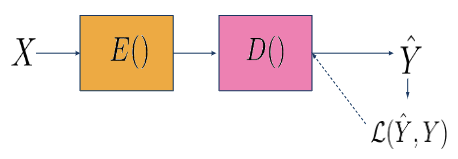
\includegraphics[width=.5\linewidth]{figures/encoder-decoder.png}
\end{figure}

\begin{itemize}
    \item Encoder function $E()$ - Represents the source as a latent encoding we cannot interpret
    \item Decoder function $D()$ - Generates a target from the latent encoding.
    \item Input sequence (source) $X=\{x_1,\dots, x_i\}$
    \item Output sequence (target) $Y=\{y_1,\dots, y_i\}$
    \item Loss over out outputs; our predicted output given our real output.
\end{itemize}

\subsection{RNNs}

\begin{figure}[H]
    \centering
    \subfigure[vanilla RNN]{\includegraphics*[trim={3px 0 0 0}, clip, width=.8\linewidth]{figures/RNN.png}}
    \subfigure[bidirectional RNN]{\includegraphics*[width=.8\linewidth]{figures/RNN-bidirectional.png}}
\end{figure}

Using a BiRNN is appropriate for encoding the source as we’re not trying to
predict the source. We have access to the whole thing at inference time. Using
a BiRNN, and reading information from both sides, allows us to gain a more
information dense representation of our sequence

We can get a hint of representation for each word and hit a representation for each word. The inner representation of each word consists of the forward direction concatentated witht he backwards direction for that particular word or particular token concatenated together.

\subsubsection{Naiive implementataion of machine translation}

\begin{figure}[H]
    \centering
    \includegraphics*[width=\linewidth]{figures/naiive-rnn.png}
\end{figure}

Given an input seqeunce we want to generate the output sequence. We get a c, the context vector, which we initialize our language model (the pink model, the decoder) which we initialize with the hidden state. The context comes from the encoder.

In the bidirectional RNN case, there are two ways that we can compute the context vector. 

\begin{enumerate}
    \item Simply take the lsat representations form the forward and backward direction and calculate them together
    \item Average across each one of those representations adn theat can form our context vector (there is a leakage here)
\end{enumerate}

The dimension of $C$ if dimensionality of the model is $d$, then we either have to set s in $R^{2d}$ or project $c$ down to $R^d$.

\subsubsection{Teacher Forcing}

\begin{figure}[H]
    \centering
    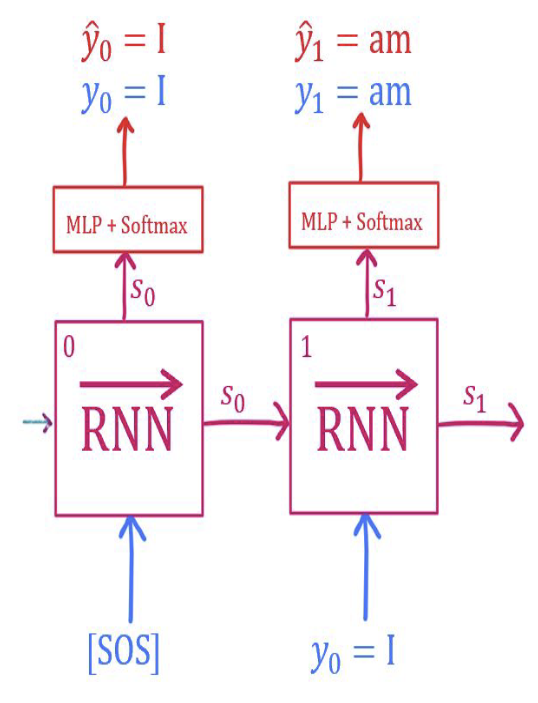
\includegraphics[width=.3\linewidth]{figures/teacher-forcing.png}
\end{figure}

Decoder is auto-regressive only during inference

During training, we use teacher forcing. We are feeding the ground truth token ot the enxt deconder cell: $S_t$ makes a prediciton, we calculate loss $\mathcal L (\hat y_t, y_t)$ then feed $y_t$ to decoder cell at $t+1$.

We use teacher forcing with a \textbf{ratio}. I.e. we well teacher force
ratio\% of time. The ratio can be 100\% (i.e. full teacher forcing), 50\%, or you
can even anneal it during training

If at timestamp $t$ the model makes a wrong prediction $\hat y_t$ with standard autoregressive modelling, if we fed this back inot decoder at call $t+1$ our model has (potentially) incorrect context. It will use this incorrect context to decode $\hat y_{t+1}$; we will likley produce another incorrect owrd. This leads to an accumulation of errors, which is difficult to optimze over.

Teacher forcing creates a phenomenon called Exposure Bias.
Exposure Bias is when the data distributions the model is conditioned on vary between training and inference. In this case, if we set teacher forcing to 100\%, then the model is never conditioned on its own predictions. So during inference, when the model uses the previously generated words as context, it is different than what it has seen in training.

\subsection{Attention}

\subsection{Transformers}

\end{document}
